
\section{Method}
Here we will presnet some basic models to solve this question independently, which includes logistic regression, svm, decision tree and random forest. At last we will introduce how to ensemble all the model together to boost our perfermances.
\subsection{Logistic Regression}
In this task, the logistic regression can solve the binary classification problems. The specific model is as following:
\begin{equation}
    P(y|x) = \sigma(y\cdot W^Tx)
\end{equation}
Once we confirm the model, we can construct some loss function to learn the parameters by stochasitc gradient descent.
\begin{equation}
    loss(y, x) = -\sum_{i=1}^{m} [y_i ln\sigma(W^Tx_i)+(1-y_i)ln(1-\sigma(W^Tx_i))]
\end{equation}
In genearlly, we can overfit the validation data because of lots of features. So we need to add some regularization term to reduce the model complexity.
So we can rewrite the loss function as:
\begin{equation}
    loss_{reg}(y,x) = loss(y, x) + \lambda W^TW
\end{equation}
Here we will explore the influence of regularization strength terms. 
\begin{figure}
    \centering
    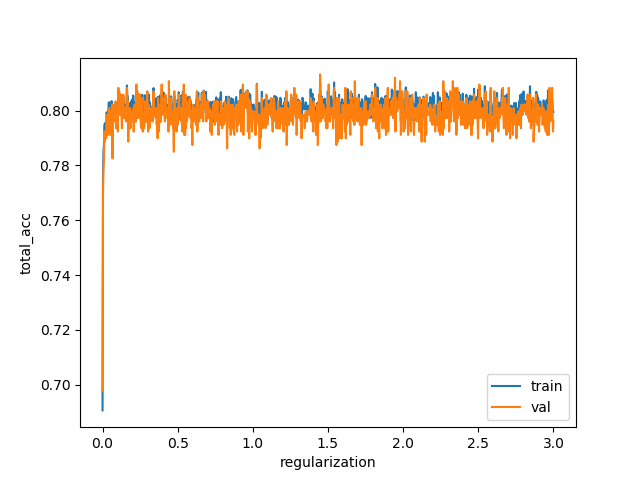
\includegraphics[width=0.5\linewidth]{img/acc_bs1_total_smote.png}
    
\end{figure}
We can see that when we set $\lambda=0.189$ to get the best perfermances.

\subsection{SVM}
The intuition of SVM\cite{SVM} is to manimize the margin, which can get more better generalization powers. Let's see mathematical equations in SVM.
\begin{align}
    min_w & \quad \frac{1}{2} W^TW \\
    s.t. &\quad y_i(W^T x_i+b) \geq 1  \quad i = 1\dots m
\end{align}

In genearlly, the data cannot be seperated in limited dimension. So we can map the data to high dimension to let it be sepearted. So we can use some kernel tricks to get better perfermances. There are several kernel function,so we will give some comparision for different kernel function.
\textbf{to post some figure in kernel function}

\subsection{Decision Tree}
The decision tree can provide a explainable model to solve problems. In this taks we have different attributes in total. We can compute the information gain to get the split results.
\begin{equation}
    Gain(D, a) = Ent(D) - \sum_{v=1}^{V} \frac{|D^v|}{|D|} Ent(D^v)
\end{equation}
In some degree, information gain can solve most of problems.But when we have lots of categories, information gain will fail. So we can use gain ratio to get more better perfermances.
\begin{align}
    &Gain\_ratio(D, a) = \frac{Gain(D,a)}{IV(a)}\\
    &IV(a) = -\sum_{v=1}^{V} \frac{|D^v|}{|D|} \log\frac{|D^v|}{|D|}
\end{align}
we always choose the most gain ratio to be our nodes. There are lost of parameters in decision tree, we will give the influence of tree depth.

% pic